\chapter{Background}

\writingbox{Hook and intro to the background. State that there are large simplifications for understanding and modelling purposes?}

TRY NOT TO MAKE THIS TOO LONG. The focus should be on your work, not what already exists. Clear and concise.

This section provides the key background knowledge that motivates the design choices and the biology behind the models developed. Whilst self-evident, the biology and theory are increasingly complex the more we explore them, and it should be noted that the mechanisms discussed are often simplified

\section{Auditory Cues and Echolocation}

Much like sonar, bats send out sound waves to reflect off of prey in an active acoustic sensing strategy called echolocation (i.e. locating with echoes). This is different from the passive sound localisation that most other mammals do, which entirely depends on external ambient sounds. The active nature of echolocation means the bat can have control and knowledge of the signal it is sending out, and so can observe changes to this signal in order to infer the location of objects, such as insects. These changes, or auditory cues, are essentially the features extracted from the returned echo for the bat's brain to infer the location, much like a typical signal processing problem.

\subsection{Auditory Cues}



\begin{figure}[H]
    \centering
    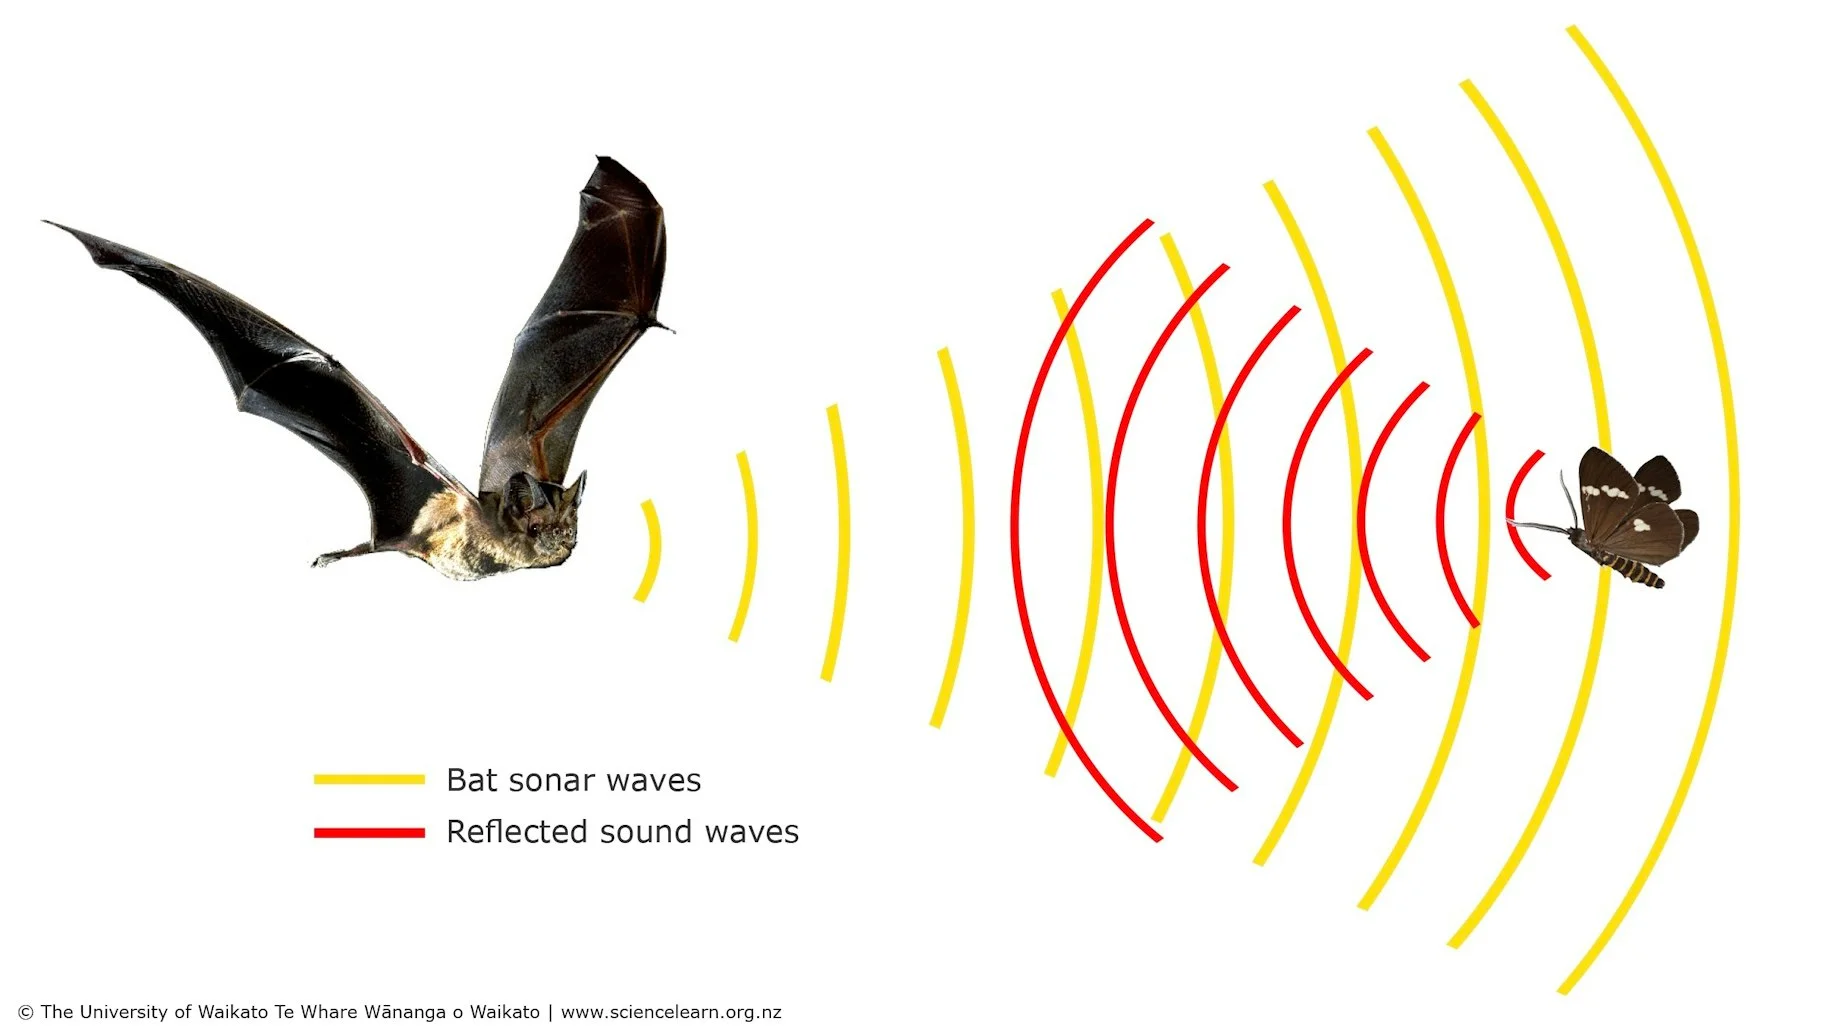
\includegraphics[width=0.72\linewidth]{2_Background/background_figures/Auditory_localisation/bat_echolocation.png}
    \caption{This diagram shows a bat, its ultrasound call, and the echo from an object, displaying the idea behind distance time of flight (ToF) cues \cite{BatHub}.}
    \label{fig:bat_echolocation}
\end{figure}



\begin{figure}[t]
    \centering
    
    % Panel A
    \begin{subfigure}[t]{0.5\textwidth}
        \textbf{\large A}\\[0.5ex]  % Forces the bold 'A' to the top left
        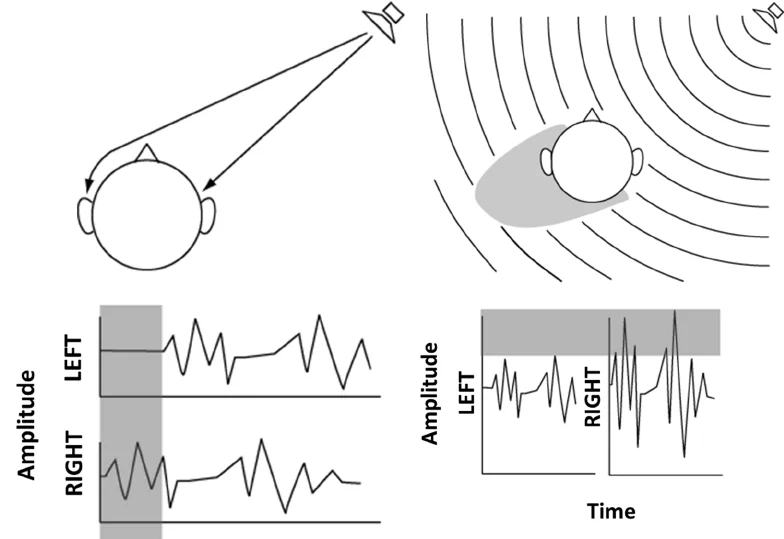
\includegraphics[height=5cm]{2_Background/background_figures/Auditory_localisation/itd_ild.png}
        \label{fig:itd_ild}
        \caption{}
    \end{subfigure}
    \hspace{0.1cm}
    % Panel B
    \begin{subfigure}[t]{0.3\textwidth}
        \textbf{\large B}\\[0.5ex]  % Forces the bold 'B' to the top left
        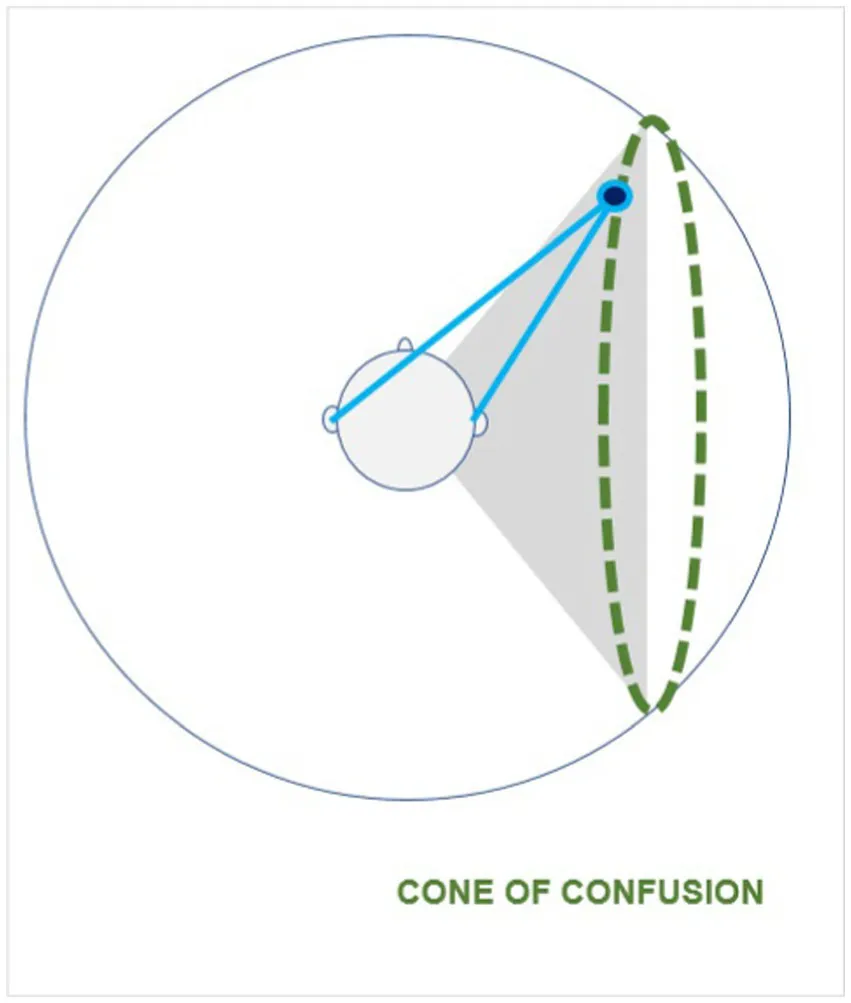
\includegraphics[height=5cm]{2_Background/background_figures/Auditory_localisation/cone.png}
        \caption{}
        \label{fig:cone}
    \end{subfigure}

    \caption{A: Interaural Time Difference (ITD) and Interaural Level Difference (ILD) \cite{Sun2015DynamicListeners}. B: Cone of confusion of constant ITD \cite{Carlini2024AuditoryReview}.}
    \label{fig:azimuth_cues}
\end{figure}



\begin{figure}[t]
    \centering
    
    % Panel A
    \begin{subfigure}[t]{0.45\textwidth}
        \textbf{\large A}\\[0.5ex]  % Forces the bold 'A' to the top left
        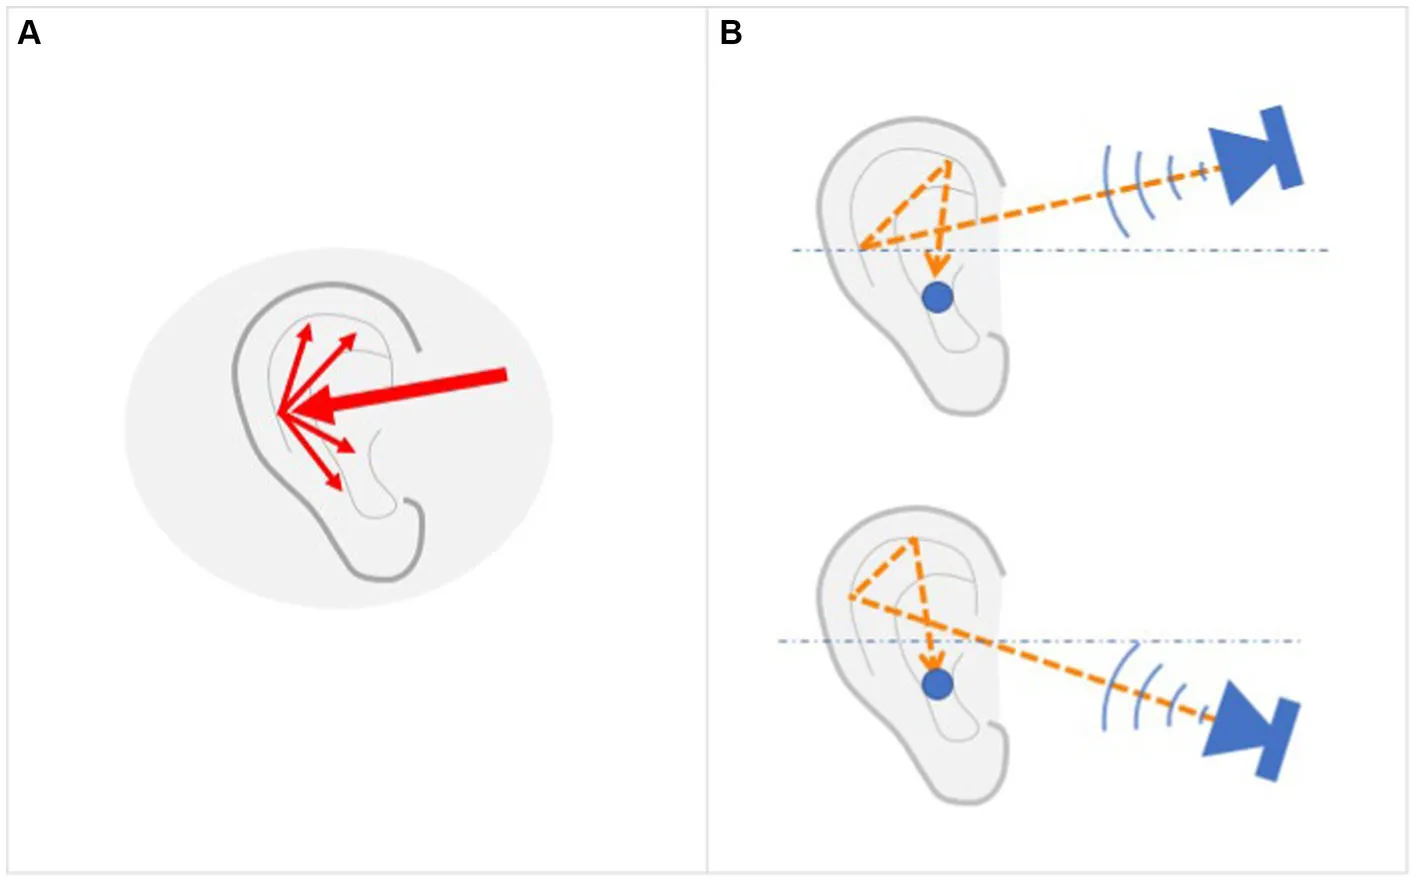
\includegraphics[height=4cm]{2_Background/background_figures/Auditory_localisation/pinna_1.png}
        \label{fig:pinna}
        \caption{}
    \end{subfigure}
    \hspace{0.1cm}
    % Panel B
    \begin{subfigure}[t]{0.45\textwidth}
        \textbf{\large B}\\[0.5ex]  % Forces the bold 'B' to the top left
        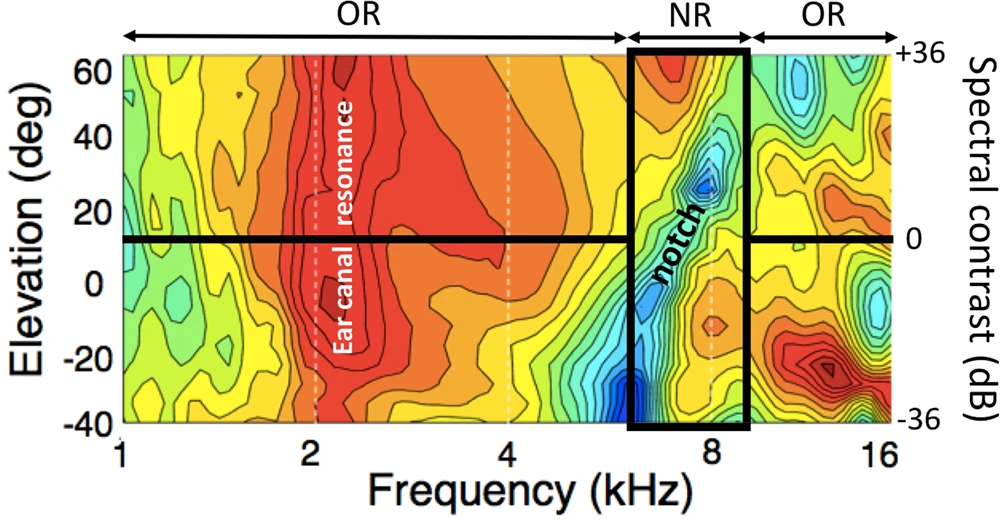
\includegraphics[height=4cm]{2_Background/background_figures/Auditory_localisation/pinna_map.png}
        \caption{}
        \label{fig:pinna_map}
    \end{subfigure}

    \caption{A: Mechanics of Head Related Transfer Function (HRTF) due to the pinna \cite{Carlini2024AuditoryReview}. B: Color-coded HRTFs for elevation. High gain in red and low gain in blue. OR: outer region. NR: notch region \cite{Zonooz2019SpectralElevation}.}
    \label{fig:elevation_cues}
\end{figure}

\begin{figure}[H]
    \centering
    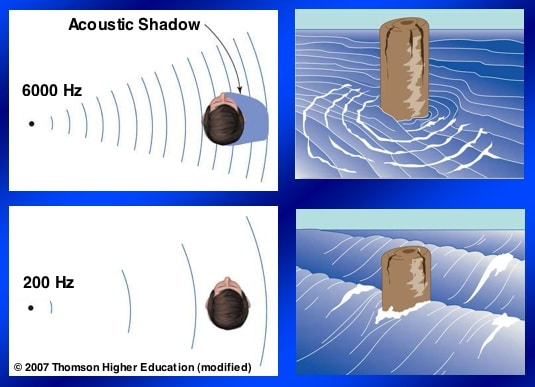
\includegraphics[width=0.72\linewidth]{2_Background/background_figures/Auditory_localisation/waves.png}
    \caption{Head shadow effect is primarily active for high frequency sounds that have short wavelengths and meet resistance and absorption when encountering the head. Low frequency sounds have long wavelengths, are able to diffract around the head, and therefore have less significant interaural intensity differences \cite{HowLocalization}. YOU DONT MODEL THIS, LIKELY REMOVE}
    \label{fig:waves}
\end{figure}


\section{Principles of Passive Auditory Localization}
Auditory localisation is the computational process by which an organism reconstructs the three-dimensional coordinates (azimuth, elevation, and distance) of an acoustic source from a pair of one-dimensional time-series waveforms. Unlike the visual system, where spatial coordinates map directly onto a two-dimensional retinal topology, the sensory periphery of the auditory system (the cochlea) organizes inputs purely by frequency. Consequently, spatial coordinates are completely implicit and must be actively computed by the central nervous system.

In passive localization—the mechanism used by humans and non-echolocating animals—the observer relies entirely on ambient sound fields. This section outlines the primary physical cues used to resolve these spatial coordinates, establishing the baseline signal-processing problems that biological neural architectures must solve.

\subsection{Horizontal Localization (Azimuth)}
Localization within the horizontal plane relies predominantly on binaural cues, which compare the differences between the acoustic signals arriving at the left and right ears.

\begin{itemize}
    \item \textbf{Interaural Time Difference (ITD):} When a sound source is located off-center, the acoustic wavefront travels a longer path to reach the farther ear. This path length difference creates a arrival time delay, geometrically approximated as:
    \begin{equation}
        \text{ITD} = \frac{r}{v}(\theta + \sin\theta)
    \end{equation}
    where $r$ is the acoustic radius of the head, $v$ is the speed of sound, and $\theta$ is the azimuth angle. ITD is highly effective for low-frequency signals where the acoustic wavelength ($\lambda$) is significantly larger than the dimensions of the head ($\lambda > 2r$).
    
    \item \textbf{Interaural Phase Difference (IPD):} For continuous, ongoing sounds, the ITD manifests as a continuous phase shift between the cycles of the incoming waveforms. Neurons track this via cycle-by-cycle phase-locking. However, if the sound frequency is high enough that the wavelength is shorter than the distance between the ears ($\lambda < 2r$), multiple acoustic cycles fit between the two ears. This introduces a catastrophic \textit{phase ambiguity} where a single IPD can correspond to multiple distinct physical angles.
    
    \item \textbf{Interaural Level Difference (ILD):} When the acoustic wavelength is shorter than the diameter of the head ($\lambda < 2r$), the sound wave cannot easily diffract around the structure. The head acts as an acoustic barrier, casting an "acoustic shadow" over the contralateral (farther) ear. This attenuates the sound amplitude at the far ear, creating an intensity difference. Because it relies on acoustic shadowing, ILD is highly effective for high-frequency sounds.
\end{itemize}

The classic transition between relying on low-frequency ITD and high-frequency ILD is known as the \textit{Duplex Theory} of sound localization. 

\subsection{Vertical Localization (Elevation)}
Binaural cues alone are insufficient for unambiguous 3D localization. A specific ITD or ILD value does not define a single coordinate in space, but rather a three-dimensional hyperbolic surface centered on the interaural axis—a geometric ambiguity known as the \textbf{Cone of Confusion}. A sound originating from $30^{\circ}$ in front of the observer produces identical ITD/ILD values to a sound originating from $150^{\circ}$ behind or above.

To resolve elevation and break the symmetry of the Cone of Confusion, the auditory system relies on monaural spectral cues. The asymmetrical, convoluted cartilage of the outer ear (the pinna) acts as an acoustic directional filter. As sound waves strike the ridges of the pinna, they reflect and interfere destructively or constructively depending on their angle of incidence. This introduces direction-specific spectral peaks and notches into the frequency profile.

This spatial filtering is mathematically formalized as the \textbf{Head-Related Transfer Function (HRTF)}, which captures the frequency-dependent changes in amplitude and phase imposed by the torso, head, and pinna geometry as a function of azimuth ($\theta$), elevation ($\phi$), and frequency ($f$):
\begin{equation}
    H(f, \theta, \phi) = \frac{P_{\text{eardrum}}(f, \theta, \phi)}{P_{\text{free-field}}(f)}
\end{equation}


\section{Biological Foundations of Echolocation}
The objective of this section is not to provide an exhaustive anatomical survey of the chiropteran brain, but rather to isolate the core computational principles, structural constraints, and functional logic found in biological auditory systems. By abstracting these biological mechanisms into discrete signal-processing blocks, we establish a direct architectural framework for the neuromorphic model developed in Section [X]. Consequently, biological components are evaluated strictly on their input-output transformations and their capacity to resolve spatial ambiguities.

\subsection{Bats and Echolocation: The Signal}
Echolocation is an active acoustic sensing strategy where an organism emits a self-generated sonar pulse and extracts three-dimensional environmental data from the returning reflections. While passive localization relies entirely on external ambient sounds, active echolocation grants the observer control over the initial signal's emission time ($t=0$), amplitude, spectral composition, and directional focus.

Microchiroptera (echolocating microbats) predominantly utilize two distinct classes of ultrasonic vocalizations, often combined within a single pulse to exploit their complementary signal-processing advantages:

\begin{itemize}
    \item \textbf{Frequency-Modulated (FM) Sweeps:} These signals feature a rapid downward or upward linear or hyperbolic shift in frequency over a brief duration (typically 1--5~ms). Because an FM sweep distributes acoustic energy across a broad spectral bandwidth, it serves as an excellent tool for \textit{temporal target ranging}. When the broad-bandwidth echo returns, it provides sharp, non-ambiguous cross-correlation peaks in time, allowing the bat to calculate distance down to millimeter precision and resolve surface textures.
    \item \textbf{Constant-Frequency (CF) Tones:} These signals consist of a long, single-frequency acoustic tone sustained for up to tens of milliseconds. A pure CF tone concentrates acoustic energy into an incredibly narrow bandwidth, making it highly insensitive to fine temporal variations but exceptionally sensitive to velocity-induced frequency shifts. Bats use CF components to exploit the \textit{Doppler Effect}, calculating the relative radial velocity of prey based on the frequency shift between the emitted call ($f_0$) and the returning echo ($f_e$).
\end{itemize}

Given that the model developed in this project focuses on a single-pulse, full-loop spatial localization task containing distance, azimuth, and elevation metrics, the primary input data pipeline is designed to mimic the wideband temporal properties of an FM target-ranging sweep.

\subsection{Biological Neurons: The Basics of Biological Computation}
Unlike conventional digital processors that transmit continuous 32- or 64-bit floating-point numbers across centralized buses, biological neural networks compute using asynchronous, binary, event-driven signals called \textit{action potentials} or \textit{spikes}. 

A biological neuron can be mathematically abstracted as a lossy, charge-integrating capacitor bounded by a non-linear voltage threshold. The computational cycle relies on three core tenets:
\begin{enumerate}
    \item \textbf{Temporal and Spatial Summation:} Incoming spikes arrive via synapses along the dendritic tree. Each spike injects a minute charge, generating a localized Post-Synaptic Potential (PSP). These potentials decay exponentially over time (temporal leak) but summate together if they arrive in close temporal proximity or across multiple spatial channels simultaneously.
    \item \textbf{Threshold and Refractoriness:} If the integrated membrane potential reaches a critical voltage threshold ($V_{th}$), the cell undergoes a rapid, regenerative depolarization event, discharging a fixed-amplitude, 1~ms binary spike down its axon. Immediately following this event, the neuron enters a \textit{refractory period} where its threshold is drastically raised, enforcing a physical ceiling on the maximum firing frequency of the cell.
    \item \textbf{Synaptic Weighting and Plasticity:} The influence of an upstream spike on a downstream neuron is governed by its synaptic strength (weight). These weights are dynamic, adapting over time based on the relative timing of pre- and post-synaptic activity---a foundational principle for biological learning and temporal pattern recognition.
\end{enumerate}

\subsubsection{The Critical Computational Role of Inhibition}
In conventional artificial neural networks (ANNs), negative weights simply scale incoming numbers downward. In biological spiking networks, however, \textit{inhibitory synapses} serve active, structurally diverse computational functions that go far beyond basic scaling:
\begin{itemize}
    \item \textbf{Forward Gating and Precision Timing:} Inhibitory inputs can act as hyperpolarizing shunts that instantly suppress excitability. By arriving fractions of a millisecond after an excitatory input, feedforward inhibition creates an incredibly narrow "temporal window" during which a neuron is capable of firing. This mechanism is vital for sub-millisecond phase-locking and timing tasks.
    \item \textbf{Lateral Inhibition and Contrast Enhancement:} When an active neuron excites inhibitory interneurons that suppress its immediate spatial neighbors, it sharpens the network's tuning profile. This lateral suppression prevents signal saturation, enforces sparse coding, and allows the network to isolate peak signals out of dense, noisy background fields.
    \item \textbf{Feedback Inhibition and Gain Control:} By looping a neuron's output back onto itself via an inhibitory interneuron, biological circuits implement localized automatic gain control. This keeps neural firing rates stable across massive variations in input sound intensity, such as the transition from a deafening emitted pulse to a faint, attenuated echo.
\end{itemize}
The interplay between fast excitation and structured lateral inhibition forms the absolute mathematical foundation for the Continuous Attractor Neural Network (CANN) architectures implemented later in this report.


\subsection{Neurobiology of the Auditory Pathways}
To transition from a raw, physical acoustic echo to a localized spatial coordinate, the microchiropteran brain processes signals through an intricate, parallelized network of subcortical nuclei. This architecture functions as an assembly line of specialized computing units, where raw sensory streams are progressively filtered, duplicated, and cross-correlated. 

Figure~\ref{fig:overall_pathway} illustrates the structural topology of the ascending auditory system of \textit{Microchiroptera}. This specific wiring diagram serves as the structural blueprint for the synthetic SNN model developed in this work. Rather than building a single monolithic network, our modeling approach directly mirrors this biological division of labor: a uniform front-end peripheral network handles sensory digitization, which then diverges simultaneously into three parallel, feature-specific midbrain processing pipelines for distance, azimuth, and elevation extraction.

\begin{figure}[htbp]
    \centering
    % \includegraphics[width=\textwidth]{overall_pathways.pdf}
    \caption{Architectural topology of the ascending microchiropteran auditory system, illustrating the functional divergence from the cochlear nuclei into parallelized spatial mapping pathways.}
    \label{fig:overall_pathway}
\end{figure}

While current state-of-the-art biological auditory models (such as \textit{CoNNear} or the \textit{Lauscher} framework) prioritize hyper-realistic, biophysical simulations using partial differential equations to track cochlear fluid mechanics, this report focuses on an alternate engineering objective: extracting the underlying \textit{neuromorphic algorithms} required to implement an end-to-end spatial localization loop on real-time spiking hardware.

\subsection{The Auditory Frontend: Peripheral \& Hindbrain Processing}

\subsubsection{Cochlea}
The cochlea is the biomechanical transducer of the auditory system. Mechanically, it operates as a hydrodynamic frequency analyzer. Incoming acoustic pressure waves travel along the basilar membrane, which varies continuously in width and stiffness from its base to its apex. This variation generates a spatial gradient of resonance: high frequencies create peak displacements near the rigid base, while low frequencies propagate to the flexible apex. 

This spatial layout is known as \textbf{tonotopic organization}. Specialized hair cells along the membrane detect these local displacements and trigger voltage-gated channels, converting continuous fluid dynamics into asynchronous spike trains along the auditory nerve.

\paragraph{Engineering Simplifications:} For the model developed in this report, the continuous mechanical properties of the basilar membrane are simplified using a discrete, parallelized Gammatone filter bank. The continuous output of each frequency channel is then digitized into discrete binary events via an integrate-and-fire spike encoder. This eliminates computationally expensive fluid-dynamic calculations while fully preserving the foundational tonotopic mapping and phase-locking capabilities required by downstream networks.

\subsubsection{Cochlear Nuclei}
The cochlear nerve terminates directly within the Cochlear Nucleus (CN), the primary hindbrain processing station. The CN acts as the master router of the auditory system. It takes the single tonotopic spike stream from the ear and duplicates it across three major specialized sub-nuclei, each optimizing the signal for a completely different downstream computational task.

\begin{figure}[htbp]
    \centering
    % \includegraphics[width=0.7\textwidth]{cochlear_nucleus.pdf}
    \caption{Functional specialization within the Cochlear Nuclei: divergence of the tonotopic input stream into timing, transient, and spectral feature extractors.}
    \label{fig:cochlear_nucleus}
\end{figure}

\paragraph{Ventral Cochlear Nucleus (VCN):} 
The VCN handles the preservation of timing and intensity details. It is structurally bifurcated into two primary functional components:
\begin{itemize}
    \item \textbf{Anteroventral Cochlear Nucleus (AVCN):} The AVCN is dominated by \textit{spherical and globular bushy cells}. These neurons feature exceptionally massive, secure synaptic connections known as the \textit{Endbulbs of Held}. These specialized synapses exhibit minimal jitter and ultra-fast recovery times, allowing the cells to replicate the firing patterns of the auditory nerve with sub-millisecond temporal fidelity. The AVCN exists to preserve precise temporal phase and timing information, acting as the primary input engine for the binaural azimuth pathway.
    \item \textbf{Posteroventral Cochlear Nucleus (PVCN):} The PVCN is characterized by \textit{octopus and stellate cells}. Octopus cells act as global onset detectors. They possess wide dendritic trees that pool spikes across a broad range of frequency channels. When a rapid wideband signal---such as an FM echolocation sweep---strikes the periphery, these cells integrate the incoming wavefront and discharge a single, hyper-precise "onset spike." This provides a clean, unambiguous temporal anchor marking the exact arrival time of the echo, which is critical for distance calculation.
\end{itemize}

\paragraph{Dorsal Cochlear Nucleus (DCN):}
In stark contrast to the timing-focused VCN, the DCN features a highly stratified, complex internal circuitry that operates as an adaptive spectral analyzer. The DCN processes monaural spectral cues by combining direct acoustic inputs from the cochlea with inhibitory feedback from internal interneurons. 

Its primary computational objective is to extract direction-specific spectral notches and peaks imposed on the echo by the bat's pinna (the Head-Related Transfer Function). By identifying how these notches shift in frequency space, the DCN extracts a raw spectral fingerprint that maps directly to the vertical elevation of the target. This pre-filtered spectral landscape is passed directly to the midbrain for elevation mapping.


\subsection{The Distance Pathway: Temporal Interval Arithmetic}
\label{sec:distance_pathway}
Target distance (range) estimation in active echolocation is fundamentally a problem of time-of-flight estimation. The central nervous system must calculate the temporal interval ($\Delta t$) between the broadcast of the vocalization and the arrival of the returning echo, mapping this delay to a physical distance axis where $d = \frac{v \cdot \Delta t}{2}$ ($v$ being the acoustic velocity).

\begin{figure}[htbp]
\centering
\begin{tikzpicture}[
    node distance=1.2cm and 2cm,
    block/.style={rectangle, draw=black, fill=blue!5, rounded corners, text width=4.5cm, text centered, minimum height=1cm, font=\small},
    arrow/.style={-Stealth, thick, draw=black!70}
]

% Nodes
\node (input) [block, fill=orange!5] {\textbf{Acoustic Pulse / Echo}};
\node (cochlea) [block, below=of input] {\textbf{Cochlea}\\(Gammatone Filter Bank)};
\node (pvcn) [block, below=of cochlea] {\textbf{PVCN (Octopus Cells)}\\(Absolute Onset Timestamping)};
\node (ic) [block, below=of pvcn] {\textbf{Inferior Colliculus (IC)}\\(Central Nucleus)};
\node (output) [block, fill=green!5, below=of ic] {\textbf{Temporal Interval Map}\\(Coincidence Detection / Delay Tuning)};

% Paths
\draw [arrow] (input) -- (cochlea);
\draw [arrow] (cochlea) -- (pvcn);
\draw [arrow] (pvcn) -- (ic);
\draw [arrow] (ic) -- (output);

\end{tikzpicture}
\caption{Signal routing architecture of the distance pathway, tracing onset timestamp generation to midbrain delay-tuned circuits.}
\label{fig:tikz_distance_pathway}
\end{figure}

\subsubsection{Signal Routing and Onset Extraction}
The distance pathway bypasses the complex spatial integration networks of the hindbrain, relying instead on high-speed, direct temporal encoding. The primary anchor points are the \textbf{octopus cells} within the posteroventral cochlear nucleus (PVCN). These cells act as wideband transient detectors, firing a single, jitter-free action potential precisely at the onset of both the emitted pulse and the returning echo. This pair of timestamps is transmitted directly via the lateral lemniscus to the central nucleus of the \textbf{Inferior Colliculus (IC)}, the primary midbrain integration hub.

\subsubsection{Asymmetric Sequential Facilitation}
Within the IC, temporal intervals are converted into a spatial topographic representation via \textit{delay-tuned neurons} (specifically categorized as FM-FM neurons). These cells are highly non-linear coincidence detectors: they remain completely silent when stimulated by the pulse or echo alone, but exhibit a massive, facilitated response when the two signals arrive at a specific, characteristic delay interval.

The underlying neural mechanism relies on \textbf{asymmetric sequential facilitation}, modeled as follows:
\begin{enumerate}
    \item \textbf{The Pulse Delay Line:} The initial timestamp representing the emitted pulse triggers an internal neural delay circuit. This is biophysically achieved through long axonal transmission loops, slow-acting metabotropic inhibitory paths, or sustained, tuned hyperpolarization-rebound mechanisms.
    \item \textbf{The Echo Direct Line:} The subsequent timestamp representing the returning echo travels along a fast, direct feedforward pathway with minimal propagation latency.
    \item \textbf{Coincidence Detection:} If the physical time-of-flight of the echo perfectly matches the internal propagation delay of the pulse channel, the two electrical inputs arrive at the post-synaptic IC neuron simultaneously. This concurrent depolarization breaches the firing threshold, discharging a localized spike.
\end{enumerate}

\subsubsection{The Simmons-Suga Hyperacuity Debate}
When implementing this architecture computationally, a core engineering trade-off must be addressed regarding how these delays are organized, famously highlighted by the academic debate between James Simmons and Nobuo Suga:
\begin{itemize}
    \item \textbf{The Suga Model (Discrete Templates):} Asserts that distance is represented by an array of rigidly pre-wired, discrete neural delay lines. Neurons are mapped to specific millisecond intervals (e.g., 1~ms, 2~ms, 3~ms), meaning resolution is fundamentally bounded by the density and step-size of the physical templates.
    \item \textbf{The Simmons Model (Hyperacuity Phase-Correlation):} Proves that behavioral tracking displays a hyperacuity down to tens of nanoseconds, arguing that the auditory system performs an active, continuous cross-correlation or phase-coherent spectral analysis that goes far beyond discrete millisecond delay lines.
\end{itemize}
\paragraph{Engineering Resolution:} To balance biological plausibility with neuromorphic hardware constraints, the model implemented in Section~[X] utilizes a discrete feedforward array inspired by the Suga template model, but couples it with a Continuous Attractor Neural Network (CANN) readout layer to interpolate between discrete channels and achieve hyper-precise target localization.


\subsection{The Azimuth Pathway: Binaural Disparity Processing}
\label{sec:azimuth_pathway}
Azimuth localization requires the extraction of subtle spatial disparities across two separated acoustic receptors. However, because microchiropteran bats possess exceptionally small interaural distances (often less than 1--2~cm), they confront extreme physical constraints that fundamentally alter how they process binaural cues compared to larger mammals.

\begin{figure}[htbp]
\centering
\begin{tikzpicture}[
    node distance=1.2cm and 1.5cm,
    block/.style={rectangle, draw=black, fill=blue!5, rounded corners, text width=3.2cm, text centered, minimum height=1cm, font=\small},
    midblock/.style={rectangle, draw=black, fill=purple!5, rounded corners, text width=3.2cm, text centered, minimum height=1cm, font=\small},
    arrow_exc/.style={-Stealth, thick, draw=green!60!black},
    arrow_inh/.style={-Stealth, thick, draw=red!70!black, dashed},
    arrow_std/.style={-Stealth, thick, draw=black!70}
]

% Left Side Peripheral Nodes
\node (ear_l) [block, fill=orange!5] {\textbf{Left Ear (Ipsilateral)}};
\node (avcn_l) [block, below=of ear_l] {\textbf{Left AVCN}\\(Spherical Bushy Cells)};
\node (lso_l) [midblock, below=of avcn_l] {\textbf{Left LSO}\\(Binaural Comparator)};

% Right Side Peripheral Nodes
\node (ear_r) [block, fill=orange!5, right=of ear_l] {\textbf{Right Ear (Contralateral)}};
\node (avcn_r) [block, below=of ear_r] {\textbf{Right AVCN}\\(Spherical Bushy Cells)};
\node (mntb_r) [block, fill=red!5, below=of avcn_r] {\textbf{Right MNTB}\\(Glycinergic Interneurons)};

% Central Midbrain Hub
\node (ic) [block, fill=green!5, below=of lso_l, xshift=2.35cm] {\textbf{Inferior Colliculus (IC)}\\(Azimuth Coordinate Map)};

% Left Paths
\draw [arrow_std] (ear_l) -- (avcn_l);
\draw [arrow_exc] (avcn_l) -- node[left, font=\scriptsize, text=green!50!black] {Excitation (+)} (lso_l);

% Right Paths
\draw [arrow_std] (ear_r) -- (avcn_r);
\draw [arrow_exc] (avcn_r) -- (mntb_r);

% Cross-line Subtractive Inhibition Path
\draw [arrow_inh] (mntb_r) -- node[above, font=\scriptsize, text=red!70!black] {Inhibition (-)} (lso_l);

% Final Output Projections
\draw [arrow_std] (lso_l) |- (ic);
\draw [arrow_std] (mntb_r) |- (ic);

\end{tikzpicture}
\caption{Binaural subtractive wiring diagram of the horizontal azimuth pathway. The LSO isolates spatial coordinates by subtracting contralateral MNTB inhibition from ipsilateral AVCN excitation.}
\label{fig:tikz_azimuth_pathway}
\end{figure}

\subsubsection{The Microbat ITD Contradiction}
In human audition, Interaural Time Differences (ITDs) processed in the Medial Superior Olive (MSO) serve as the dominant horizontal localization metric. For a microbat, however, a sound source at $90^{\circ}$ azimuth produces a maximum physical ITD of only approximately $30$ to $50~\mu\text{s}$. Given that standard biological membrane constants operate on millisecond timescales, traditional Jeffress-style delay-line networks struggle to robustly resolve these microsecond time-of-flight differences. Consequently, while phase-locking exists for low frequencies, the bat's azimuth pipeline relies overwhelmingly on intensity disparities.

\subsubsection{LSO-MNTB Lateral Integration Architecture}
To overcome this temporal barrier, the bat leverages high-frequency \textbf{Interaural Level Differences (ILDs)} processed within the \textbf{Lateral Superior Olive (LSO)} and the \textbf{Medial Nucleus of the Trapezoid Body (MNTB)}. This subcortical circuit transforms minute intensity differences into a robust, high-contrast rate-code via an elegant subtractive lateral inhibition framework:

\begin{equation}
    I_{\text{LSO}} = f\left( W_{\text{ipsi}} \cdot X_{\text{ipsi}} - W_{\text{contra}} \cdot Y_{\text{MNTB}}(X_{\text{contra}}) \right)
\end{equation}

\begin{enumerate}
    \item \textbf{Ipsilateral Excitation:} Spherical bushy cells in the AVCN directly excite the LSO on the same side as the acoustic input.
    \item \textbf{Contralateral Inhibition:} Spherical bushy cells in the opposite AVCN project across the midline to excite the MNTB. The MNTB contains glycinergic interneurons that convert this signal into a powerful, ultra-fast inhibitory input to the contralateral LSO.
    \item \textbf{Binaural Subtraction:} The LSO acts as a physical comparator. If a sound originates from the far left, the left LSO receives strong ipsilateral excitation and weak contralateral inhibition, resulting in a high firing rate. If the sound shifts to the right, the contralateral inhibition overpowers the cell, completely silencing its output.
\end{enumerate}

This subtractive architecture produces a monotonic, highly sensitive sigmoid tuning curve of spike counts relative to azimuthal angle, which is subsequently projected up to the Inferior Colliculus for integration into the full spatial map.

\subsection{The Elevation Pathway: Monaural Spectral Mapping}
\label{sec:elevation_pathway}
Vertical localization cannot be solved using binaural disparity metrics because a purely horizontal displacement can yield identical ITD and ILD values anywhere along the surface of the "Cone of Confusion." To resolve the elevation angle, the auditory system must pivot from binaural comparison to monaural signal analysis, decoding the passive spectral filtering imposed by the environment.

\begin{figure}[htbp]
\centering
\begin{tikzpicture}[
    node distance=1.2cm and 2cm,
    block/.style={rectangle, draw=black, fill=blue!5, rounded corners, text width=4.5cm, text centered, minimum height=1cm, font=\small},
    arrow/.style={-Stealth, thick, draw=black!70}
]

% Nodes
\node (input) [block, fill=orange!5] {\textbf{Acoustic Wavefront}};
\node (pinna) [block, below=of input] {\textbf{Pinna Acoustic Filter}\\(HRTF Spectral Fingerprint)};
\node (dcn) [block, below=of pinna] {\textbf{DCN (Fusiform Cells)}\\(Spectral Notch Extraction)};
\node (vnll) [block, below=of dcn] {\textbf{VNLL}\\(Transient Relay Block)};
\node (ic) [block, fill=green!5, below=of vnll] {\textbf{Inferior Colliculus (Deep Layers)}\\(Vertical Coordinate Mapping)};

% Paths
\draw [arrow] (input) -- (pinna);
\draw [arrow] (pinna) -- (dcn);
\draw [arrow] (dcn) -- (vnll);
\draw [arrow] (vnll) -- (ic);

\end{tikzpicture}
\caption{Monaural spectral routing architecture of the elevation pathway, converting physical acoustic notches into deep collicular spatial locations.}
\label{fig:tikz_elevation_pathway}
\end{figure}

\subsubsection{The Pinna as a Directional Filter}
As an active echolocator moves through an environment, the complex, highly adapted structural topology of its outer ear (the pinna) acts as a physical acoustic filter. Incoming echoes scatter across the ridges and tragi of the pinna, causing frequency-dependent constructive and destructive interference patterns. This interaction imprints unique, highly localized spectral peaks and sharp attenuation notches into the echo waveform. Because these notches shift predictable up or down in frequency depending on the incidence angle of the incoming wave, the current frequency coordinate of the notch maps directly to a physical elevation coordinate.

\subsubsection{DCN Notch-Finding and Collicular Projection}
The primary neural engine tasked with decoding this spectral footprint is the \textbf{Dorsal Cochlear Nucleus (DCN)}. The internal layers of the DCN feature a highly specialized, layered computational circuit:
\begin{itemize}
    \item \textbf{Fusiform Cells (Principal Neurons):} These cells receive direct, tonotopic raw frequency inputs from the cochlear nerve.
    \item \textbf{Tuberculoneural/Cartwheel Cells (Inhibitory Interneurons):} These interneurons form wide lateral inhibition nets across neighboring frequency channels within the DCN.
\end{itemize}

When an echo arrives with a pinna-induced spectral notch, the frequency channels corresponding to that notch fall silent. This localized drops in excitation unburdens the neighboring fusiform cells from local lateral inhibition, causing them to fire intensely. 

This neural mechanism effectively computes the derivative of the spectral shape, transforming a raw acoustic drop in energy into a sharp, amplified neural firing peak. These notch-location signals are routed via the \textbf{Ventral Nucleus of the Lateral Lemniscus (VNLL)} directly into the deep layers of the \textbf{Inferior Colliculus}, completing the raw spatial input matrix by providing the vertical coordinate.










\section{Neuromorphic Computing}
To translate the biological processing principles of the chiropteran brain into an artificial engineering system, we must pivot from conventional von Neumann computing paradigms to neuromorphic architectures. Traditional digital processors isolate logic execution (CPUs/GPUs) from data storage (memory), communicating continuous 32-bit floating-point arrays across a shared bus at high clock frequencies. This structural separation induces the classic "von Neumann bottleneck," driving massive power dissipation during real-time, high-throughput sensory tasks. 

Neuromorphic computing resolves this by co-localizing memory and computation within parallel networks of event-driven, sub-threshold processing units. This section develops the mathematical and algorithmic foundation of spiking networks, establishing the exact computational primitives used to implement our active echolocation loop.

\subsection{Computing with Spikes}

\subsubsection{Spikes and Encoding}
In standard Artificial Neural Networks (ANNs), information is encoded as a continuous static variable representing neuron activation or firing rate. In contrast, Spiking Neural Networks (SNNs) communicate via sparse, asynchronous binary signals:
\begin{equation}
    s(t) = \sum_{k} \delta(t - t_k)
\end{equation}
where $\delta(t)$ is the Dirac delta function and $t_k$ represents the exact firing timestamp of the $k$-th spike. 

This formulation yields two distinct methods for data representation:
\begin{itemize}
    \item \textbf{Rate Coding:} Information is mapped to the average frequency of spikes over an extended temporal window. While robust to noise, rate coding is highly inefficient for fast, dynamic control loops because it requires integration over time, introducing significant processing latency.
    \item \textbf{Temporal Coding:} Information is encoded within the exact arrival time or relative phase of individual spikes (e.g., time-to-first-spike or phase-locking). 
\end{itemize}

For an echolocating bat, rate coding is physically impossible. A typical ultrasonic echo returns and passes across the sensory epithelium in less than 3~ms. At this microsecond timescale, an individual neuron only has the opportunity to discharge one or two action potentials. The biological architecture is therefore fundamentally forced to rely on \textit{temporal coding}, optimizing for high-speed edge detection and transient timing rather than statistical frequency averages.

\subsubsection{Neurons: Mathematical Implementations}
To simulate biological cells efficiently on digital silicon, we abstract continuous membrane biophysics into discrete phenomenological equations.

The primary workhorse of SNN design is the \textbf{Leaky Integrate-and-Fire (LIF)} neuron model. The sub-threshold membrane potential $V(t)$ is governed by a first-order linear differential equation:
\begin{equation}
    \tau_m \frac{dV(t)}{dt} = -(V(t) - V_{\text{rest}}) + R \cdot I(t)
  \label{eq:lif}
\end{equation}
where $\tau_m = RC$ is the membrane time constant, $V_{\text{rest}}$ is the resting baseline voltage, $R$ is the membrane resistance, and $I(t)$ is the incoming synaptic current. When $V(t) \ge V_{\text{th}}$, the neuron fires a binary event $s(t)=1$ and is instantaneously reset to a lower potential $V_{\text{reset}}$. Mathematically, the LIF neuron behaves as an adaptive spatiotemporal low-pass filter.

To capture frequency-selective properties natively, we also consider the \textbf{Resonate-and-Fire (RF)} neuron model. Unlike the monotonic integration of the LIF model, an RF neuron models a sub-threshold dampening oscillator using a complex-valued differential state:
\begin{equation}
    \frac{dz(t)}{dt} = (\psi + i\omega)z(t) + I(t)
\end{equation}
where $\psi$ defines the damping constant and $\omega$ represents the cell's natural resonant frequency. An RF neuron acts as a native spatiotemporal bandpass filter, allowing individual nodes to lock directly onto specific ultrasonic frequencies without requiring cascaded architectural layers.

\subsubsection{Neuronal Structures: Computational Analogies}
By arranging these basic neuron blocks into structured topologies, we can replace expensive digital signal processing (DSP) algorithms with implicit, zero-power neural mechanics:

\begin{itemize}
    \item \textbf{Coincidence Detection vs. Cross-Correlation:} In standard signal processing, calculating an echo delay requires executing an expensive discrete cross-correlation convolution:
    \begin{equation}
        R_{xy}(\tau) = \int_{-\infty}^{\infty} x(t)y(t+\tau) \, dt
    \end{equation}
    In an SNN, an array of parallel LIF neurons paired with asymmetric synaptic delays executes this cross-correlation implicitly. The membrane potential performs spatial and temporal summation; it fires a spike if and only if the inputs align perfectly in time. The mathematical integral is replaced by the passive physical physics of charge integration.
    
    \item \textbf{Spikes as Samples (Monte Carlo and Bayesian Inference):} Instead of transmitting explicit 32-bit probability distribution matrices to manage tracking uncertainties, an SNN treats a population of spikes as a stochastic Monte Carlo sampler. The presence or density of sparse spikes across a coordinate array acts as a direct, non-parametric representation of a probability density function. Bayesian updating is reduced to simple post-synaptic charge summation.
    
    \item \textbf{RF Banks vs. Fast Fourier Transforms (FFT):} Standard digital sonar systems calculate a rolling discrete Fourier transform to map frequencies. A parallel bank of Resonate-and-Fire neurons, tuned across the bat's ultrasonic bandwidth, extracts these exact frequency bins continuously in real time, converting spectral analysis into a parallelized time-domain event stream.
    
    \item \textbf{The "Switches" Argument (Logic Gates Analogy):} In von Neumann architectures, a logic gate is a static, space-bound switch that continuously draws current to maintain or transition voltage levels, regardless of whether data is changing. In a neuromorphic network, a neuron is a \textit{spatiotemporal switch}. It executes computation and consumes dynamic power only at the exact instant an incoming spike event arrives. If the environment is silent, the network draws practically zero power, decoupling processing energy from clock speed and tying it strictly to real-world data entropy.
\end{itemize}

\subsection{Continuous Attractor Neural Networks (CANN)}
While feedforward networks extract raw sensory coordinates, they are highly sensitive to sensor noise and environmental clutter. To smooth, stabilize, and track these spatial metrics, we deploy Continuous Attractor Neural Networks (CANNs).

A CANN is a recurrently wired neural population that maintains a stable localized "bump" of neural activity in the absence of sustained external stimulation. This is achieved via a \textit{local-excitation, global-inhibition} wiring scheme: neighboring neurons with similar spatial tuning excite one another, while globally projecting interneurons suppress the wider network.

\begin{itemize}
    \item \textbf{Line Attractor Models:} Map linear variables such as target distance (range). The recurrent weight matrix is symmetric and translationally invariant along a single axis, locking the neural activity bump to a specific distance coordinate and smoothly shifts its position as the echo delay changes linearly.
    \item \textbf{Ring Attractor Models:} Map cyclical angular variables such as azimuth. The topology loops back onto itself seamlessly ($0^{\circ} = 360^{\circ}$), maintaining a singular spatial coordinate vector across the horizontal plane.
\end{itemize}

Computationally, CANNs act as native non-linear filters. They track a continuous state variable, interpolate between discrete physical neuron channels (resolving the Suga template limitation), and reject multi-target noise by enforcing a strict winner-take-all activity topology.

\subsection{Spiking Neural Networks and Deep Learning}
While the frontend pathways of our model rely on fixed, biologically derived wiring templates, the final sensorimotor fusion layer must adapt dynamically to multi-modal data. This requires integrating SNNs with modern deep learning optimization techniques.

The primary mathematical hurdle when training SNNs is the non-differentiable nature of the threshold step-function. The derivative of a spike event is zero everywhere except at the exact threshold crossing, where it becomes infinite:
\begin{equation}
    \frac{\partial s(t)}{\partial V(t)} = \delta(V(t) - V_{\text{th}})
\end{equation}
This discontinuous derivative completely blocks standard gradient-descent algorithms such as Backpropagation Through Time (BPTT).

To bypass this barrier, we utilize **surrogate gradients**. During the forward execution pass, the network uses the exact, non-linear biological step threshold to preserve binary hardware efficiency. During the backward optimization pass, however, the non-differentiable delta function is substituted with a smooth, continuous approximation (such as a fast sigmoid or arctangent derivative), as illustrated in Figure~\ref{fig:surrogate_gradient}:
\begin{equation}
    \frac{\partial \tilde{s}(t)}{\partial V(t)} = \frac{1}{\left(1 + \gamma |V(t) - V_{\text{th}}|\right)^2}
\end{equation}
where $\gamma$ is a hyperparameter controlling the slope of the surrogate curve. This architecture is implemented programmatically using the \textit{snnTorch} framework, allowing the final readout network to learn non-linear sensorimotor mappings using automated, data-driven optimization.

\begin{figure}[htbp]
    \centering
    % \includegraphics[width=0.6\textwidth]{surrogate.pdf}
    \caption{The surrogate gradient optimization paradigm: replacing the non-differentiable biological step function with a smooth, continuous derivative during backpropagation.}
    \label{fig:surrogate_gradient}
\end{figure}

\subsection{Neuromorphic Hardware Compatibility}
To prove the industrial viability of our echolocation model, the complete simulation architecture is designed from the ground up to respect the strict physical execution constraints of commercial neuromorphic processors, such as the \textbf{Intel Loihi} research chip.

Intel Loihi operates as an asynchronous, many-core silicon fabric executing a discrete-time, event-driven mesh network. To ensure our algorithmic simulation can compile directly onto this class of physical hardware without modifications, our software enforces four rigid constraints:
\begin{enumerate}
    \item \textbf{Quantized/Fixed-Point Arithmetic:} Loihi does not possess floating-point arithmetic units (ALUs). Membrane dynamics, synaptic weights, and decay constants are implemented strictly using 8-bit or 24-bit fixed-point integer state tracking.
    \item \textbf{Strict Local Recurrence:} All synaptic updates and weight variables must rely entirely on data accessible locally within the core or individual compartment (e.g., local membrane voltage and local spike timing). Global, non-local network parameters are strictly forbidden during runtime execution.
    \item \textbf{Synchronized Discrete-Time Steps:} The continuous biological differential equations are discretized into unified, integer-driven execution steps ($t \to t+1$), mapping perfectly to the synchronized execution cycles of hardware network-on-chip routers.
\end{enumerate}

---

\section{Current Biomimetic Models of Echolocatory Bats}
To evaluate the originality and contribution of the model developed in this report, we must contextualize it within the existing landscape of biomimetic auditory frameworks. Current state-of-the-art architectures generally split into two isolated, non-overlapping domains:

\subsection{Biophysical Auditory Models}
Advanced mammalian peripheral simulators, such as the \textbf{CoNNear} framework (Verhulst et al.) or the \textbf{Lauscher} simulation engine, prioritize hyper-realistic anatomical fidelity. CoNNear replaces traditional, cascaded transmission-line models of the cochlea with a parallelized convolutional neural network (CNN) architecture capable of predicting level-dependent basilar membrane vibrations. 

While exceptionally precise, these frameworks are fundamentally engineered for high-performance computing clusters. They rely on dense, deep matrices of 32-bit floating-point numbers executed on high-power graphics processing units (GPUs). Because they lack sparse, binary event execution mechanics, they are structurally incompatible with real-time, low-power edge robotics or event-driven neuromorphic silicon.

\subsection{Neuromorphic VLSI Circuits}
Conversely, early neuromorphic pioneers (such as Horiuchi, Shi, and Koch) developed analog Very Large Scale Integration (VLSI) microchips that successfully emulated isolated subcortical pathways. These included dedicated hardware architectures modeling the subtractive ILD processing mechanics of the LSO or hard-wired delay lines simulating the auditory midbrain.

While these analog chips achieved sub-milliwatt power efficiency, they suffer from two major engineering limitations:
\begin{itemize}
    \item \textbf{Structural Fragmentation:} Each chip isolates a single sensory metric. Prior research lacks an integrated, multi-pathway architecture capable of unifying distance, azimuth, and elevation processing simultaneously from a single sensory input stream.
    \item \textbf{Algorithmic Rigidity:} Traditional analog VLSI layouts are hard-wired down to the physical transistor level, lacking the programmatic adaptability to train or fine-tune multi-modal sensorimotor fusion layers using automated deep learning optimization frameworks.
\end{itemize}

\subsection{The Research Gap and Originality of This Project}
The model developed in this project directly targets the unaddressed intersection between these two domains. The key original contributions of this work are summarized as follows:

\begin{enumerate}
    \item \textbf{End-to-End Functional Integration:} We present the first single-pulse echolocation simulation that unifies parallelized distance (temporal delay lines), azimuth (binaural subtractive ILD), and elevation (monaural DCN notch filtering) pipelines into a single cohesive, functional architecture.
    \item \textbf{Hardware-Compatible Hybrid Topology:} The framework bridges hard-wired biological structural constraints (such as the CANN line attractor) with data-driven neural plasticity (an SNN readout trained via surrogate gradients in \textit{snnTorch}), while operating entirely under the integer, localized, event-driven constraints required for immediate deployment onto neuromorphic processors like Intel Loihi.
\end{enumerate}














